\section{Simulation Studies}\label{section:simulations}
In this section, we examine the finite-sample performance of the proposed HIPM and WoW testing procedures. Our numerical analysis is organized into three parts. First, we investigate the validity of the permutation-based test by evaluating the Type I error rate and statistical power of both HIPM and WoW using a synthetic dataset. Second, we compare our methods with existing methods from the literature. Finally, we demonstrate the practical utility of the proposed framework through an application to a mortality dataset.

\subsection{Empirical Comparison Between HIPM and WoW}\label{subsection:hipm_wow_comparison}

We compare the use of HIPM and WoW within our permutation-based test by analysing the Type I error and the power in several simulated settings, considering both parametric and nonparametric data-generating processes, in settings that satisfy the assumptions of Theorem~\ref{theorem:perm_consistency_dlip} and in settings that do not, notably $\X = \R$, but are still of practical interest. We consider the following baselines for parametric and nonparametric models.
\begin{enumerate}
\item Parametric model that fulfills the assumptions:
\[
Q^1 = \mathcal{L}(\tilde P), \qquad \tilde P| \tilde \mu = \mathrm{Beta}( \tilde \mu, 1- \tilde \mu), \qquad \tilde \mu \sim \mathrm{Beta}(a_0 = 1, b_0 = 1);
\]
\item Parametric model that does not fulfill the assumptions:
\[
Q^1 = \mathcal{L}(\tilde P), \qquad \tilde P| \tilde \mu = \mathcal{N}(\tilde \mu, \sigma^2 = 1), \qquad \tilde \mu \sim \N(\mu_0 = 0, \sigma^2_0 = 1);
\]

\item Nonparametric model that fulfills the assumptions:
\[
Q^1 = \mathrm{DP}(\alpha = 1, P_0 = \mathrm{Unif}[0,1]);
\]
\item Nonparametric model that does not fulfill the assumptions:
\[
Q^1 = \mathrm{DP}(\alpha = 1, P_0 = N(0,1)),
\]
\end{enumerate}
where $\mathrm{Beta}(a,b)$ is the Beta distribution with shape parameters $a,b$, $\mathcal{N}(\mu, \sigma^2)$ is the Gaussian distribution with mean $\mu$ and variance $\sigma^2$, $\mathrm{Unif}[0,1]$ is the Uniform distribution on the interval $[0,1]$, and $\mathrm{DP}(\alpha, P_0)$ denotes the Dirichlet process with concentration $\alpha>0$ and base measure $P_0 \in \probx$. Note that if $P_0$ has full support on $\X$, $\mathrm{DP}(\alpha, P_0)$ has full weak support on $\probx$.

To investigate the behaviour of the Type I error, we simulate data $S = 1000$ times with $Q^1 = Q^2$ set equal to each of the four models above, perform our permutation-based test for both WoW and HIPM, and report the percentage of times it rejects the (correct) $H_0: Q^1 = Q^2$ for each significance level $\theta$. In each simulation, we set $n=m=n_{\text{perm}}= 100$.

The results are shown in Figure~\ref{figure:fp_wow_vs_hipm}, where we see that both WoW and HIPM control the Type I error at approximately the significance level $\theta$ across all simulation settings. We report only one of the four graphs, as the remaining graphs show no qualitative differences. Interestingly, WoW also appears to control the Type I error even though our theory does not guarantee it, and both methods behave well in unbounded settings.
\begin{figure}[H]
    \centering
      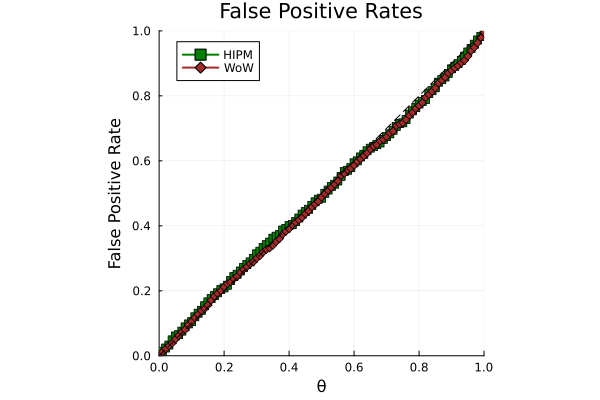
\includegraphics[width = 0.49\linewidth]{chapters/two-sample-testing/figures/wow_vs_hipm/fp_label=1_n=100_m=100_S=1000_n_perm=100.png}
    \caption{False Positive Rates for HIPM and WoW}
    \label{figure:fp_wow_vs_hipm}
\end{figure}
To investigate the power of the test, we simulate the data under the alternative hypothesis $Q^1 \neq Q^2$. For each of the four laws considered above, we associate an alternative law and estimate the power, resulting in the following four cases:
\begin{align*}
\text{A.} \quad & Q^1 = \mathcal{L}(\tilde P), \quad \tilde P| \tilde \mu = \mathrm{Beta}(\tilde \mu, 1-\tilde \mu), \quad \tilde \mu \sim \mathrm{Beta}(a_0 = 1, b_0 = 1) \\
                & Q^2 = \mathcal{L}(\tilde P), \quad \tilde P| \tilde \mu = \mathrm{Beta}(\tilde{\mu}, 1-\tilde{\mu}), \quad \tilde \mu \sim \mathrm{Beta}(a_0 = 1, b_0 = 1.5) \\[1em]
\text{B.} \quad & Q^1 = \mathcal{L}(\tilde P), \quad \tilde P| \tilde \mu = \N(\tilde \mu, \sigma^2 = 1), \quad \tilde \mu \sim \N(\mu_0 = 0, \sigma^2_0 = 1) \\
                & Q^2 = \mathcal{L}(\tilde P), \quad \tilde P| \tilde \mu = \N(\tilde \mu, \sigma^2 = 1), \quad \tilde \mu \sim \N(\mu_0 = 0, \sigma^2_0 = 1.5) \\[1em]
\text{C.} \quad & Q^1 = \mathrm{DP}(\alpha = 1, P_0 = \mathrm{Unif}[0,1]) \\
                & Q^2 = \mathrm{DP}(\alpha = 1, P_0 = \mathrm{Beta}(a_0 = 1, b_0 = 1.4)) \\[1em]
\text{D.} \quad & Q^1 = \mathrm{DP}(\alpha = 1, P_0 = \N(0,1)) \\
                & Q^2 = \mathrm{DP}(\alpha = 2, P_0 = \N(0,1))
\end{align*}
As before, we simulate data $S = 1000$ times, perform our permutation-based test for both WoW and HIPM, and report the empirical power, that is, the percentage of times it rejects the (incorrect) null $H_0: Q^1 = Q^2$, for each significance level $\theta$, setting $n=m=n_{\text{perm}}= 100$.

\begin{figure}[H]
    \centering
    \begin{subfigure}{0.49\textwidth}
        \centering
        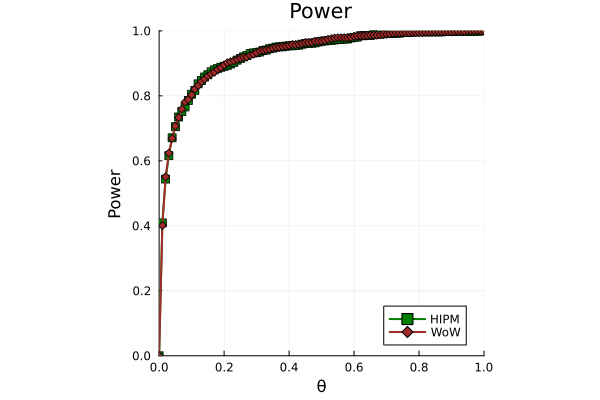
\includegraphics[width = \linewidth]{chapters/two-sample-testing/figures/wow_vs_hipm/tp_label_1=1_label_2=1_n=100_m=100_S=1000_n_perm=100.png}
        \caption{Case A}
    \end{subfigure}
    \begin{subfigure}{0.49\textwidth}
        \centering
        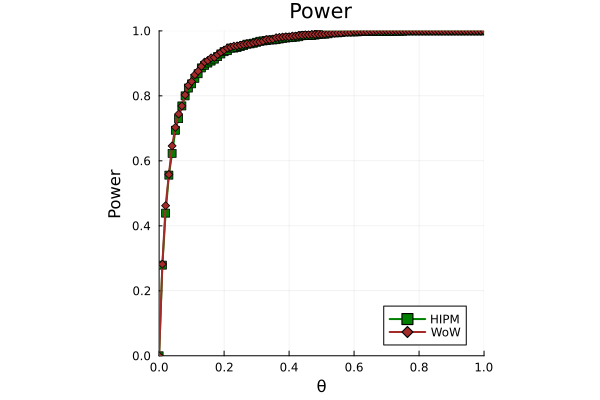
\includegraphics[width = \linewidth]{chapters/two-sample-testing/figures/wow_vs_hipm/tp_label_1=2_label_2=2_n=100_m=100_S=1000_n_perm=100.png}
        \caption{Case B}
    \end{subfigure}
    \begin{subfigure}{0.49\textwidth}
        \centering
        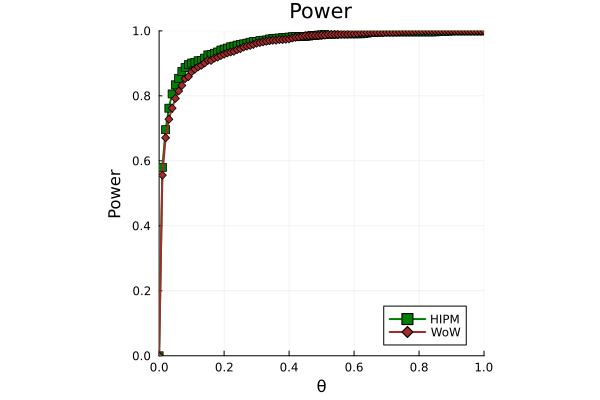
\includegraphics[width = \linewidth]{chapters/two-sample-testing/figures/wow_vs_hipm/tp_label_1=3_label_2=3_n=100_m=100_S=1000_n_perm=100.png}
        \caption{Case C}
    \end{subfigure}
    \begin{subfigure}{0.49\textwidth}
        \centering
        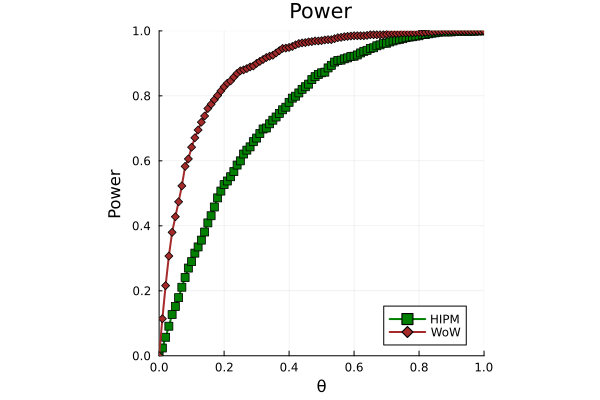
\includegraphics[width = \linewidth]{chapters/two-sample-testing/figures/wow_vs_hipm/tp_label_1=4_label_2=4_n=100_m=100_S=1000_n_perm=100.png}
        \caption{Case D}
    \end{subfigure}
    \caption{Power for WoW and HIPM}
    \label{figure:tp_wow_vs_hipm}
\end{figure}

The results presented in Figure~\ref{figure:tp_wow_vs_hipm} indicate that HIPM and WoW achieve comparable power in Cases A and B. In Case C, HIPM exhibits slightly higher power than WoW. A more pronounced difference emerges in Case D, where WoW achieves substantially higher power than HIPM. Understanding the conditions under which one method dominates the other remains an open question. One possible direction is to examine the signal-to-noise ratio of the underlying testing problem.


\subsection{Empirical comparison with existing methods}\label{subsection:comparison_of_all_methods}

Several frameworks for two-sample testing in general metric spaces have been developed in the literature. As $(\probx, \W)$ is a metric space, those methods can be specialized to that setting. We benchmark our proposed scheme against two existing methods. The first is that of \cite{dubey2019frechet}, which we refer to as the Fr\'echet test. The second is the Energy test introduced in \cite{szekely2004testing}.

The Fr\'echet test uses the concepts of Fr\'echet mean and variance for random probability measures. Recall that the mean of a real-valued random variable $X$ is the number $a \in \R$ such that
\[
a = \argmin_{a' \in \R}\E (X-a')^2.
\]
This characterization generalizes to a general metric space. In the space $(\probx,\W_2)$, the analogous notion is referred to as the Fr\'echet mean, defined as
\begin{definition}[Fr\'echet Mean]
\label{definition:Frechet_mean}
Let $Q \in \probprobx$. The Fr\'{e}chet mean is the probability measure $\mu_{F} \in \probxtwo$ defined as
\[
\mu_{F} = \argmin_{P \in \probxtwo} \E_{\widetilde{P}\sim Q} \left[\W^2_2(P, \widetilde{P})\right].
\]
\end{definition}
Accordingly, we describe the dispersion around that point, which is referred to as the Fr\'echet variance.
\begin{definition}[Fr\'echet Variance]
\label{definition:Frechet_variance}
Let $Q \in \probprobx$. The Fr\'echet variance $V_{F}$ is defined as
\[
V_{F} = \min_{P \in \probxtwo}\E_{\widetilde{P}\sim Q} \left[\W^2_2(P, \widetilde{P})\right] 
= \E_{\widetilde{P}\sim Q} \left[\W^2_2(\mu_F, \widetilde{P})\right]
\]
\end{definition}
The asymptotic theory of the Fr\'echet test is developed for bounded metric spaces under additional regularity assumptions. In the case of $\probx$, these assumptions are known to hold when the Wasserstein distance is of order $2$ and $\X$ is a compact interval of the real line. It is important to note that the Fr\'echet test targets the surrogate null hypothesis of equality of Fr\'echet means and Fr\'echet variances associated to laws of random probability measures.


The Energy test was first developed as a testing procedure for samples taking values in Euclidean spaces. It can be extended to a general metric space $(\Y,d)$, provided that the underlying space is of strongly negative type (see \cite{lyons2013distance} for a comprehensive overview).

We compare the methods in two different scenarios using the same baseline as \cite{dubey2019frechet}. In each scenario, we examine the rejection rates of each testing scheme for several pairs of laws of random probability measures. The random probability measures we consider are
\begin{equation}\label{equation:tnormal_normal_model}
\tilde P^i| \tilde \mu^{(i)} = \mathcal{N}(\tilde \mu^{(i)}, 1), \qquad \tilde \mu^{(i)} \sim  \mathcal{N}_T(\mu_{0i}, \sigma^2_{0i} , a, b),
\end{equation}
for $i = 1,2$, where $\mathcal{N}_T (\cdot, \cdot, a,b)$ denotes the truncated normal distribution on $[a,b]$. To obtain the set of pairs, we vary a parameter governing the random means. In particular, we consider the following settings:
\begin{enumerate}
\item The difference between two distributions is dictated by changing the mean parameter of the random mean, reproducing the setting of Figure~1 in \cite{dubey2019frechet}, where $Q^i$ are as in \eqref{equation:tnormal_normal_model} with $\sigma_{01} = \sigma_{02} = 0.5$, $a = -10$, $b = 10$ and
\[
\mu_{01} = 0, \qquad \mu_{02} = \delta, \qquad \delta \in [-1, 1]. 
\]
\item The difference between two distributions is dictated by changing the variance parameter of the random mean, reproducing the setting of Figure~1 in \cite{dubey2019frechet}, where $Q^i$ are as in \eqref{equation:tnormal_normal_model} with $\mu_{01} = \mu_{02} = 0$, $a = -10$, $b = 10$ and
\[
\sigma_{01} = 0.2, \qquad \sigma_{02} = 0.2\tau, \qquad  \tau \in [0, 3].
\]
\end{enumerate}
A low type I error is reflected by a low rejection rate under $H_0$, corresponding respectively to $\delta = 0$ and  $\tau = 1$. High power is reflected by a steep increase in the rejection curve away from $H_0$.

For each setting we simulate the data $S=1000$ times, perform all tests on the same data, and report the percentage of times they reject the corresponding null hypothesis. We set the hierarchical sample sizes to $n = 100$, $m = 200$. Our tests use a permutation approach with $n_{\text{perm}} = 100$ re-samples, while the Fr\'echet test uses a bootstrap approach with $n_{\text{boot}} = 100$ re-samples. For the Fr\'echet test, we work directly with samples from the Gaussian distributions rather than hierarchical samples. Results are reported in Figure~\ref{figure:rejections_mean_variance}.
\begin{figure}[H]
    \centering
    \begin{subfigure}{0.49\textwidth}
        \centering
        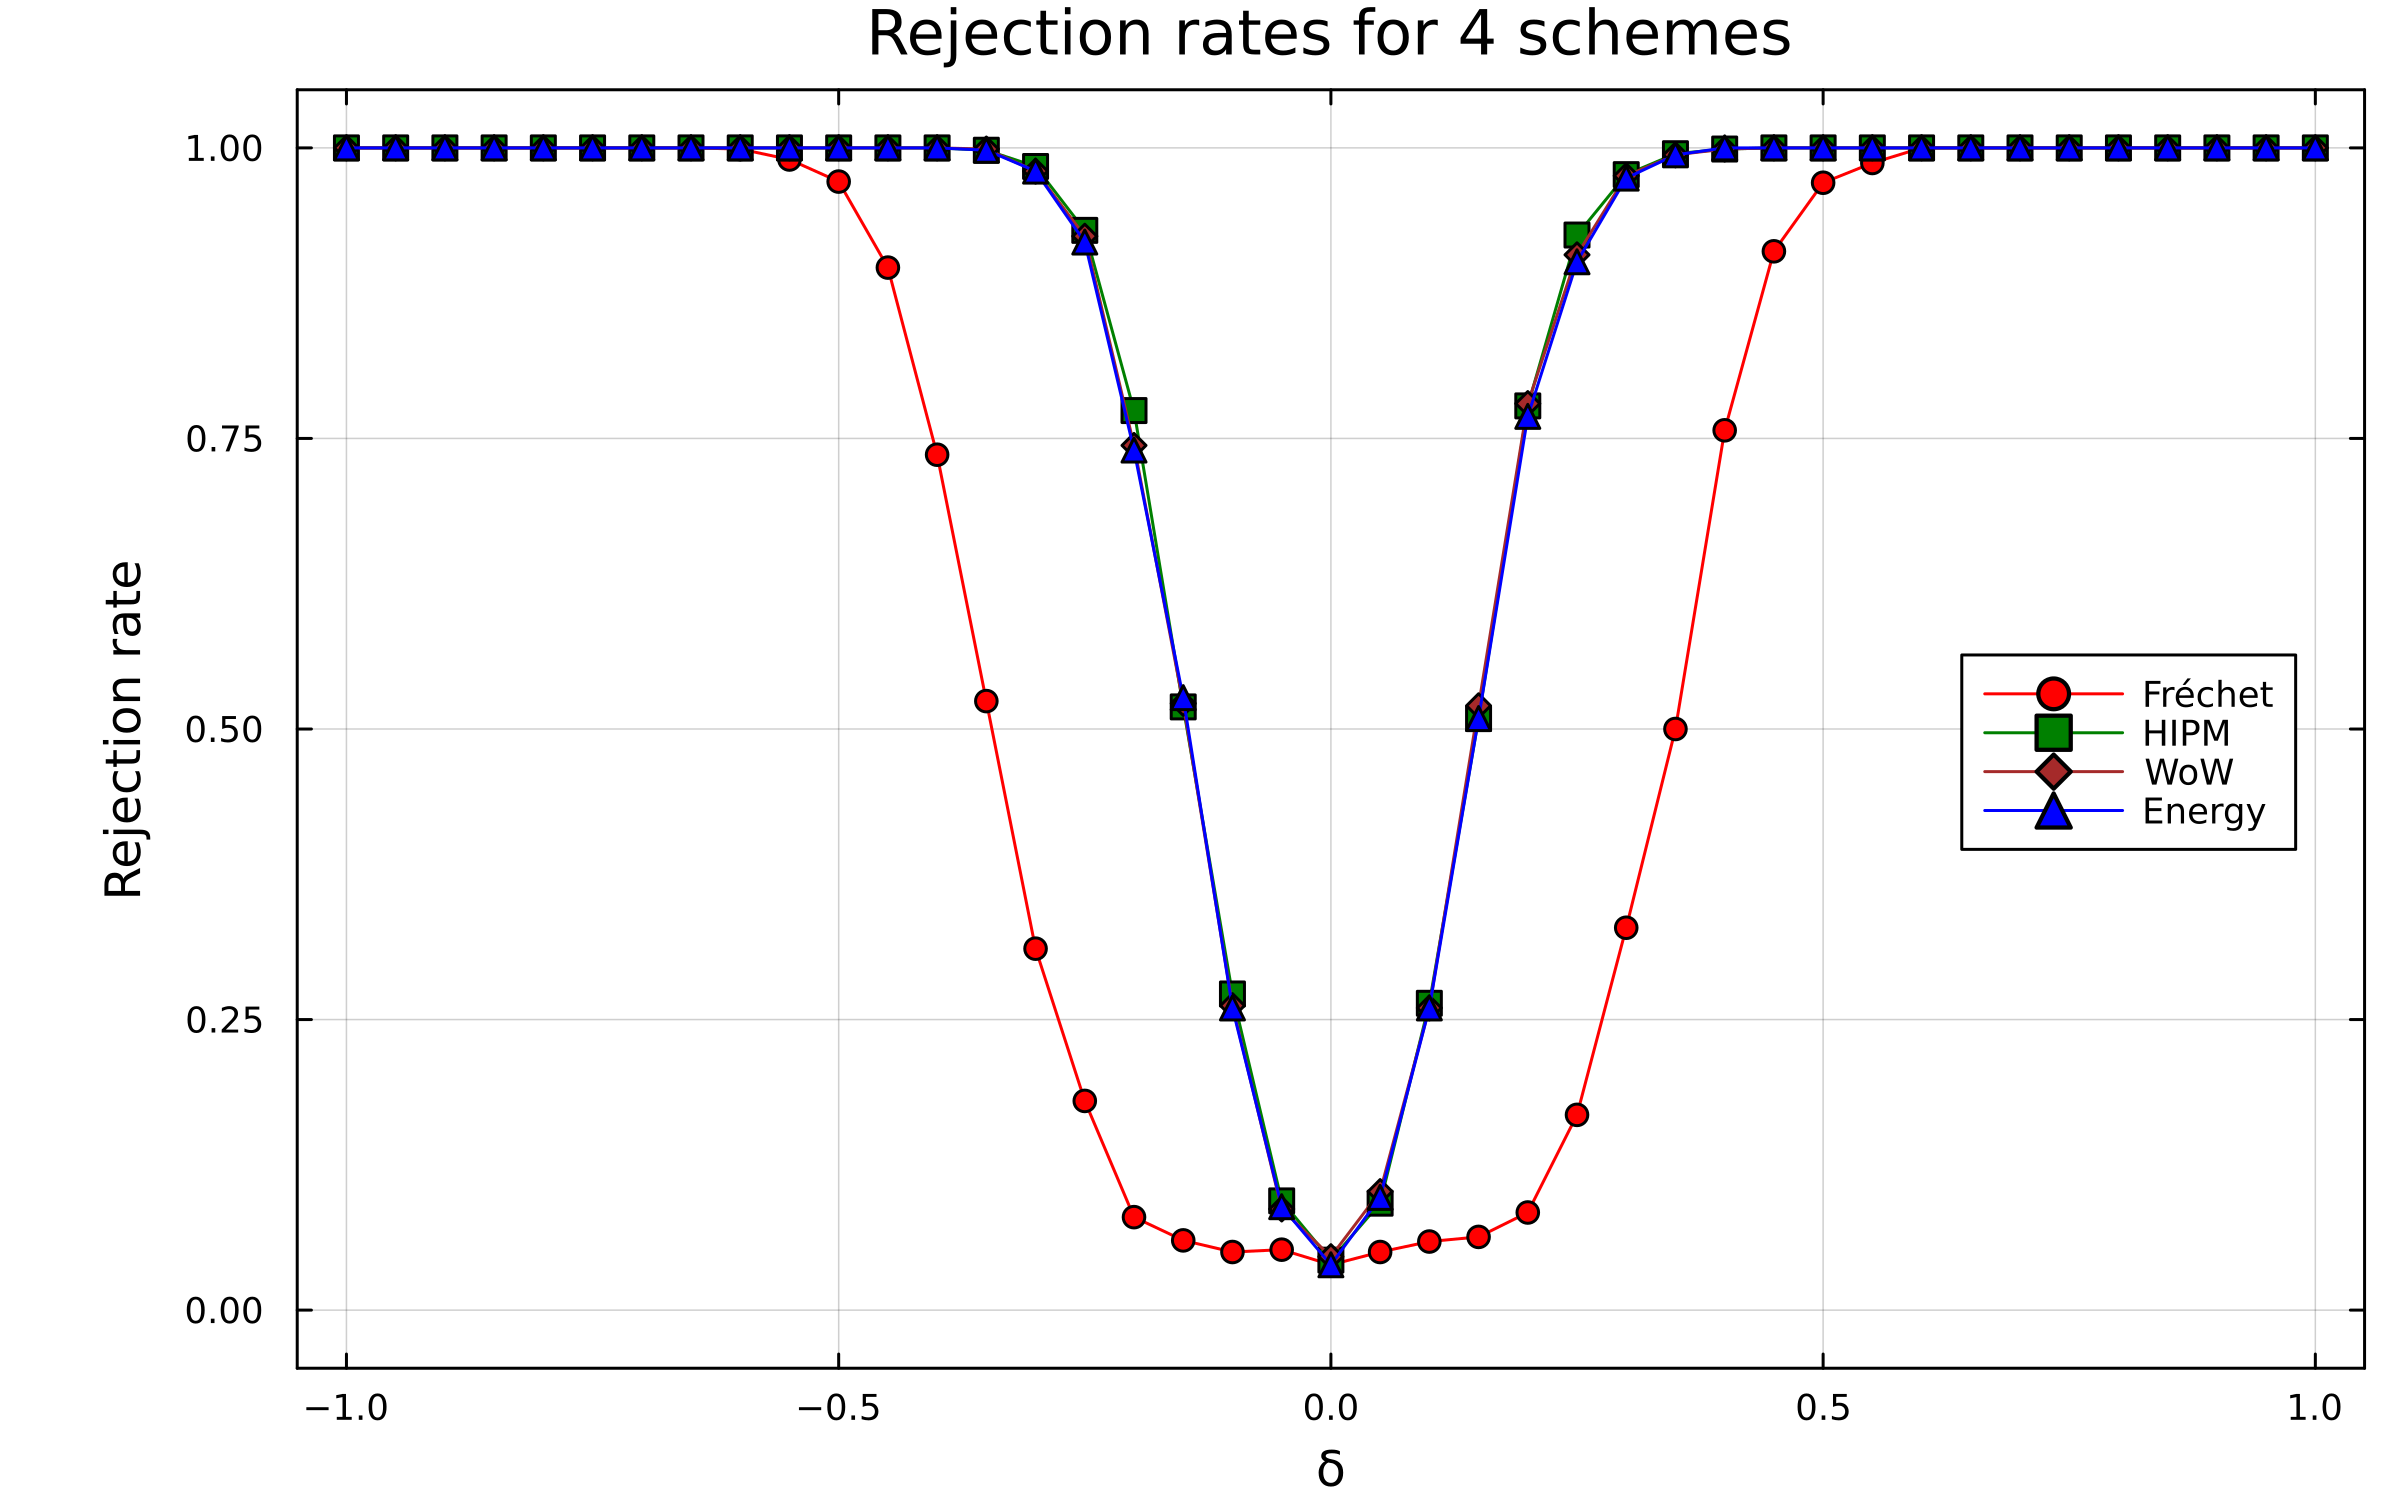
\includegraphics[width = \linewidth]{chapters/two-sample-testing/figures/all_schemes/mean_n=100_m=200_S=1000_bootstrap=false_n_samples=100.png}
    \end{subfigure}
    \begin{subfigure}{0.49\textwidth}
        \centering
        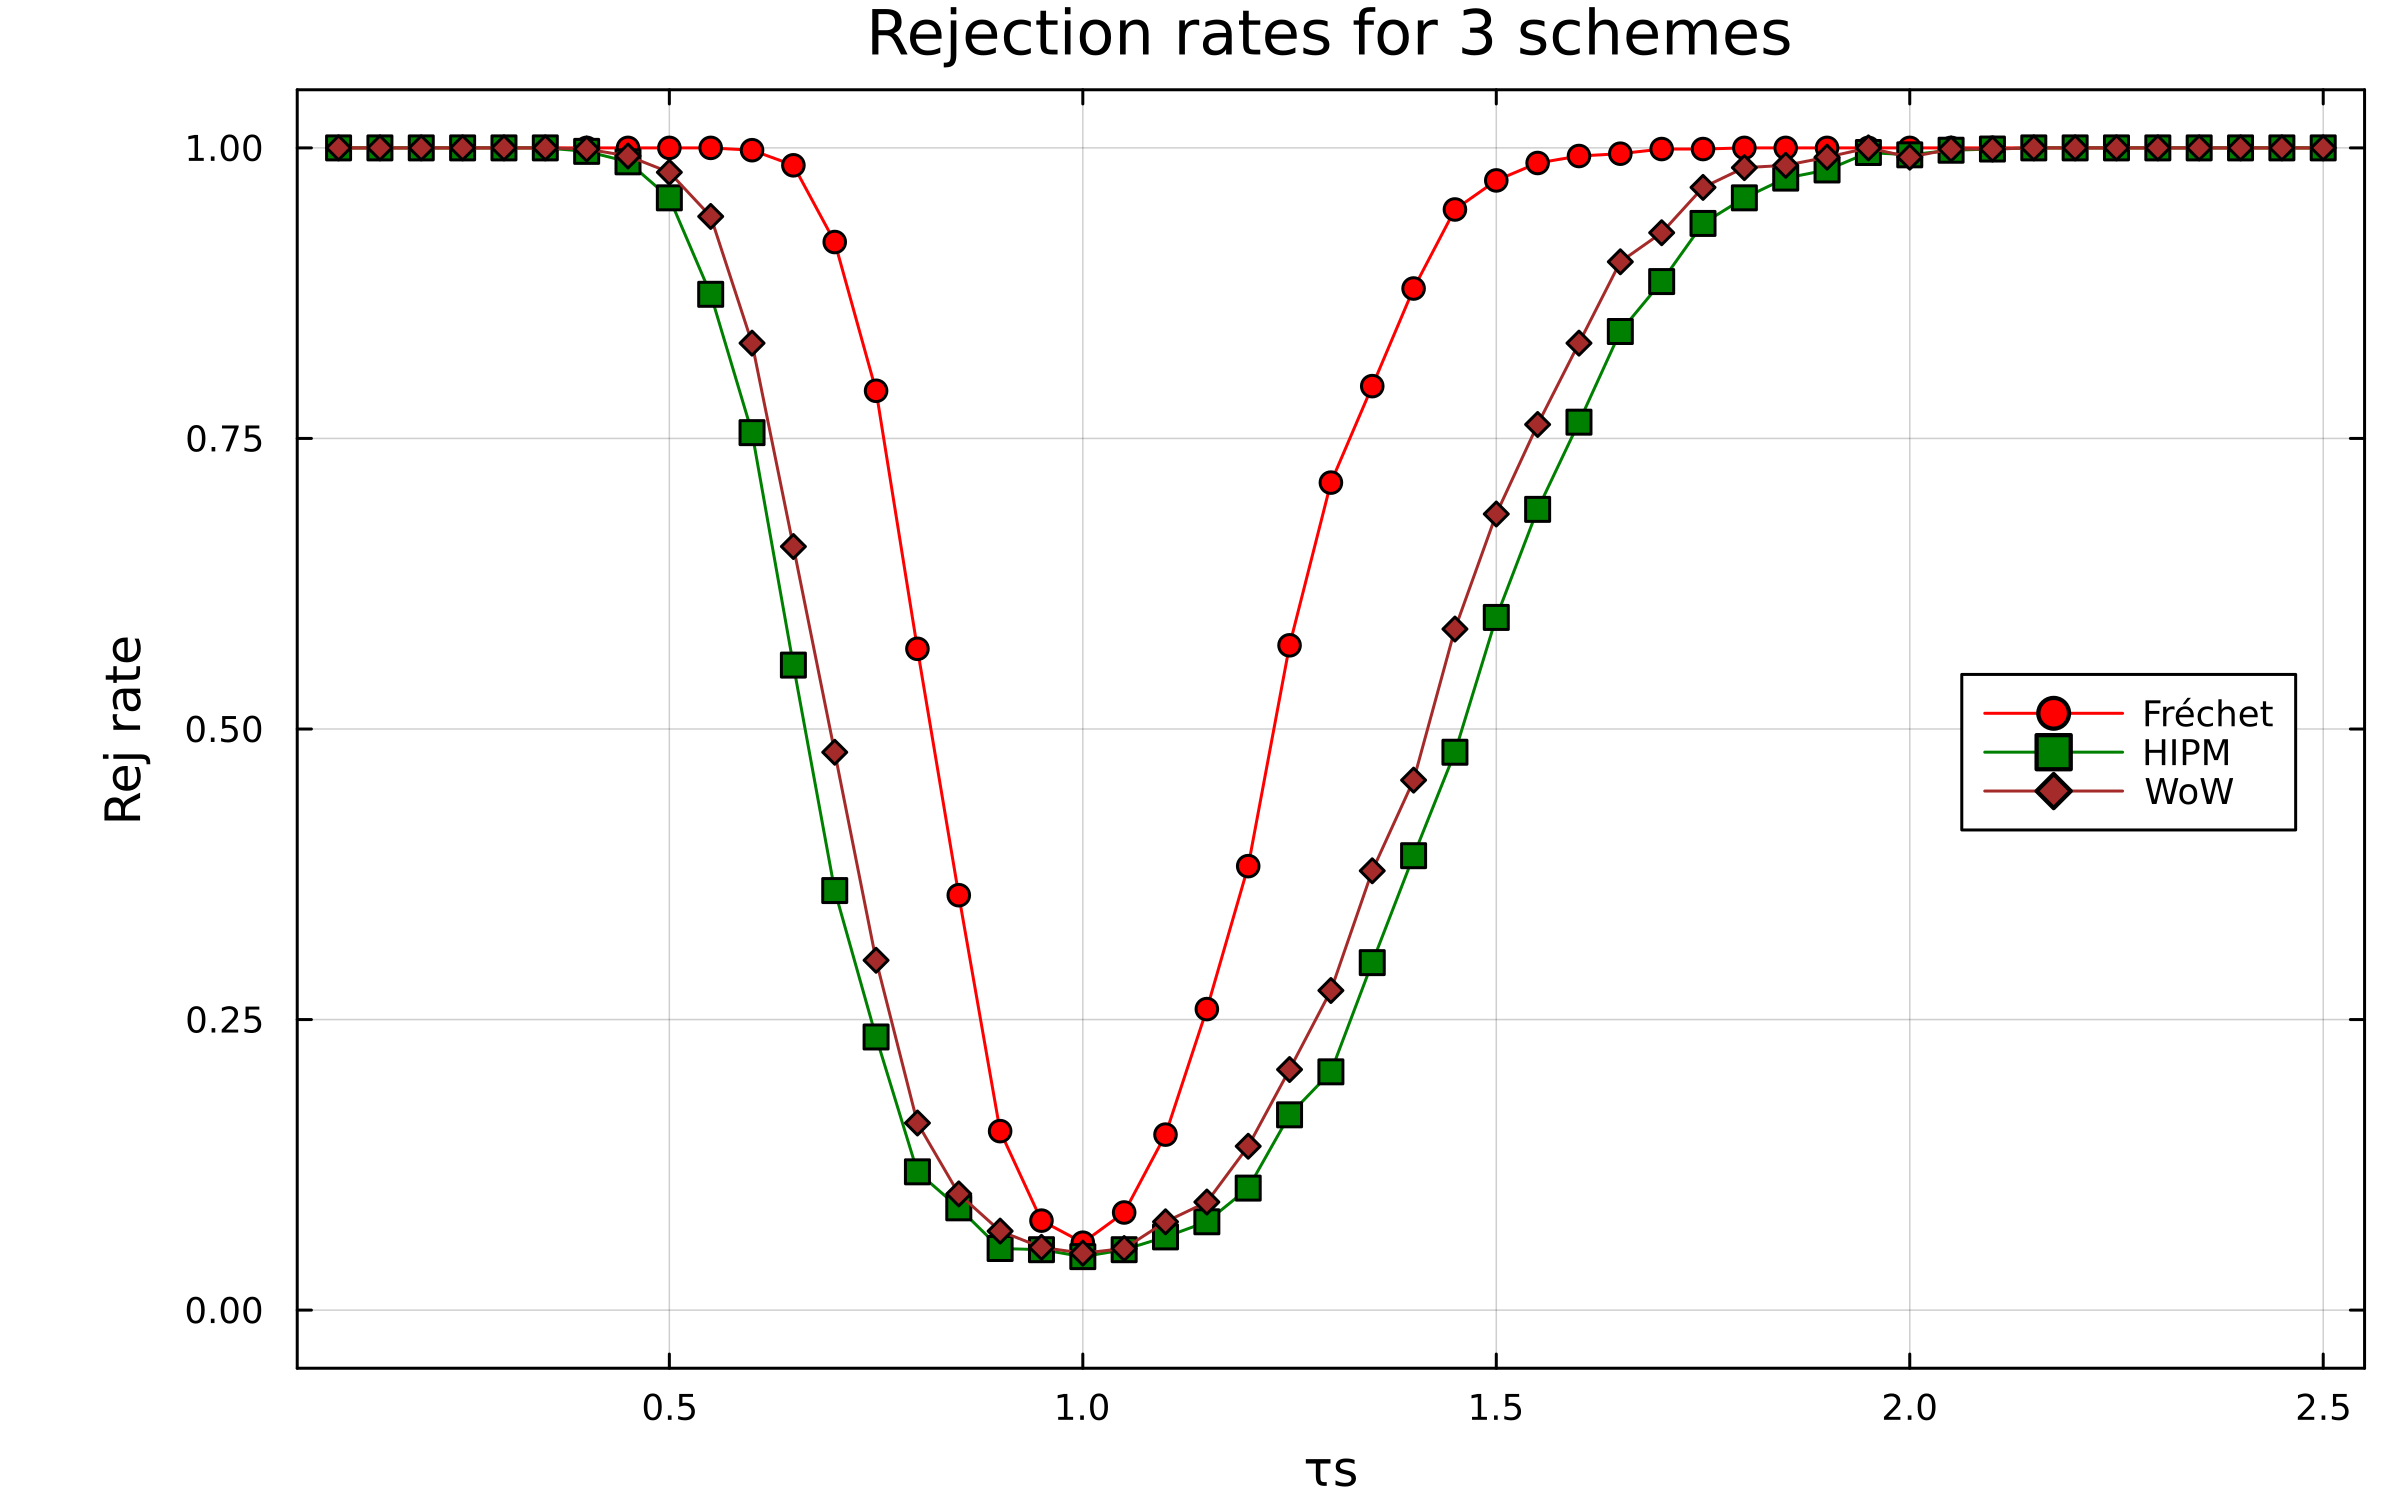
\includegraphics[width = \linewidth]{chapters/two-sample-testing/figures/all_schemes/variance_n=100_m=200_S=1000_bootstrap=false_n_samples=100.png}
    \end{subfigure}
    \caption{Rejection rates for WoW, HIPM, Fr\'echet and Energy tests}
    \label{figure:rejections_mean_variance}
\end{figure}
As seen in Figure~\ref{figure:rejections_mean_variance}, all testing schemes maintain low Type I error across both settings. When the distributions differ in mean (left plot), the Energy, WoW, and HIPM tests achieve higher power than the Fr\'echet test. In contrast, when the distributions differ in variance (right plot), the Fr\'echet test attains the highest power among all methods. Furthermore, in the variance setting, both HIPM and WoW outperform the Energy test.


The final simulation on the synthetic dataset is designed to demonstrate the necessity of distance-based testing. Note that the underlying assumption behind the Fr\'echet test is that the Fr\'echet mean and variance are sufficient to distinguish between two different laws of random probability measures. However, laws of RPMs are not always uniquely characterized by their Fr\'echet means and variances.

Indeed, we can construct a simple counterexample. Consider
\begin{align*}
   &Q^1 = \law\widetilde{P}^1 \quad \text{where} \quad \widetilde{P}^1 | \tilde{\mu} = \N\left( \widetilde{\mu}^1, 1\right), \quad \widetilde{\mu}^1 \sim \tfrac{1}{2}\delta_{-1} + \tfrac{1}{2}\delta_{1}, \\
   &Q^2 = \law \widetilde{P}^2 \quad \text{where} \quad \widetilde{P}^2 | \tilde{\mu}  = \N\left( \widetilde{\mu}^2, 1\right), \quad \widetilde{\mu}^2 \sim  \tfrac{1}{8}\delta_{-2} + \tfrac{3}{4}\delta_{0} + \tfrac{1}{8}\delta_{2},
\end{align*}
where $Q^1 \neq Q^2$, yet their associated Fr\'echet means and variances coincide (see Remark~\ref{remark:frechet_mean_variance_special_case_variance_1}).

Moreover, if we compare $Q^1$ with a mixture of $Q^1$ and $Q^2$, the resulting laws remain different while still inducing the same Fr\'echet means and variances (see Remark~\ref{remark:frechet_mean_variance_mixture_of_laws}). Specifically, letting
\[
M_\lambda = \lambda Q^1 + (1-\lambda)Q^2,
\]
we consider the family of pairs
\[
\{(Q^1, M_\lambda) : \lambda \in [0,1]\}.
\]
Note that $\lambda = 1$ corresponds to estimating the Type~I error, while other values of $\lambda$ correspond to estimating the power of the testing procedures. We consider mixtures of the two laws because, as the parameter varies, it becomes more challenging for the testing schemes to detect the presence of different laws. We plot the rejection rates in Figure~\ref{figure:counterexample}, where the simulation parameters are the same as those used in Figure~\ref{figure:rejections_mean_variance}.
\begin{figure}[H]
    \centering
    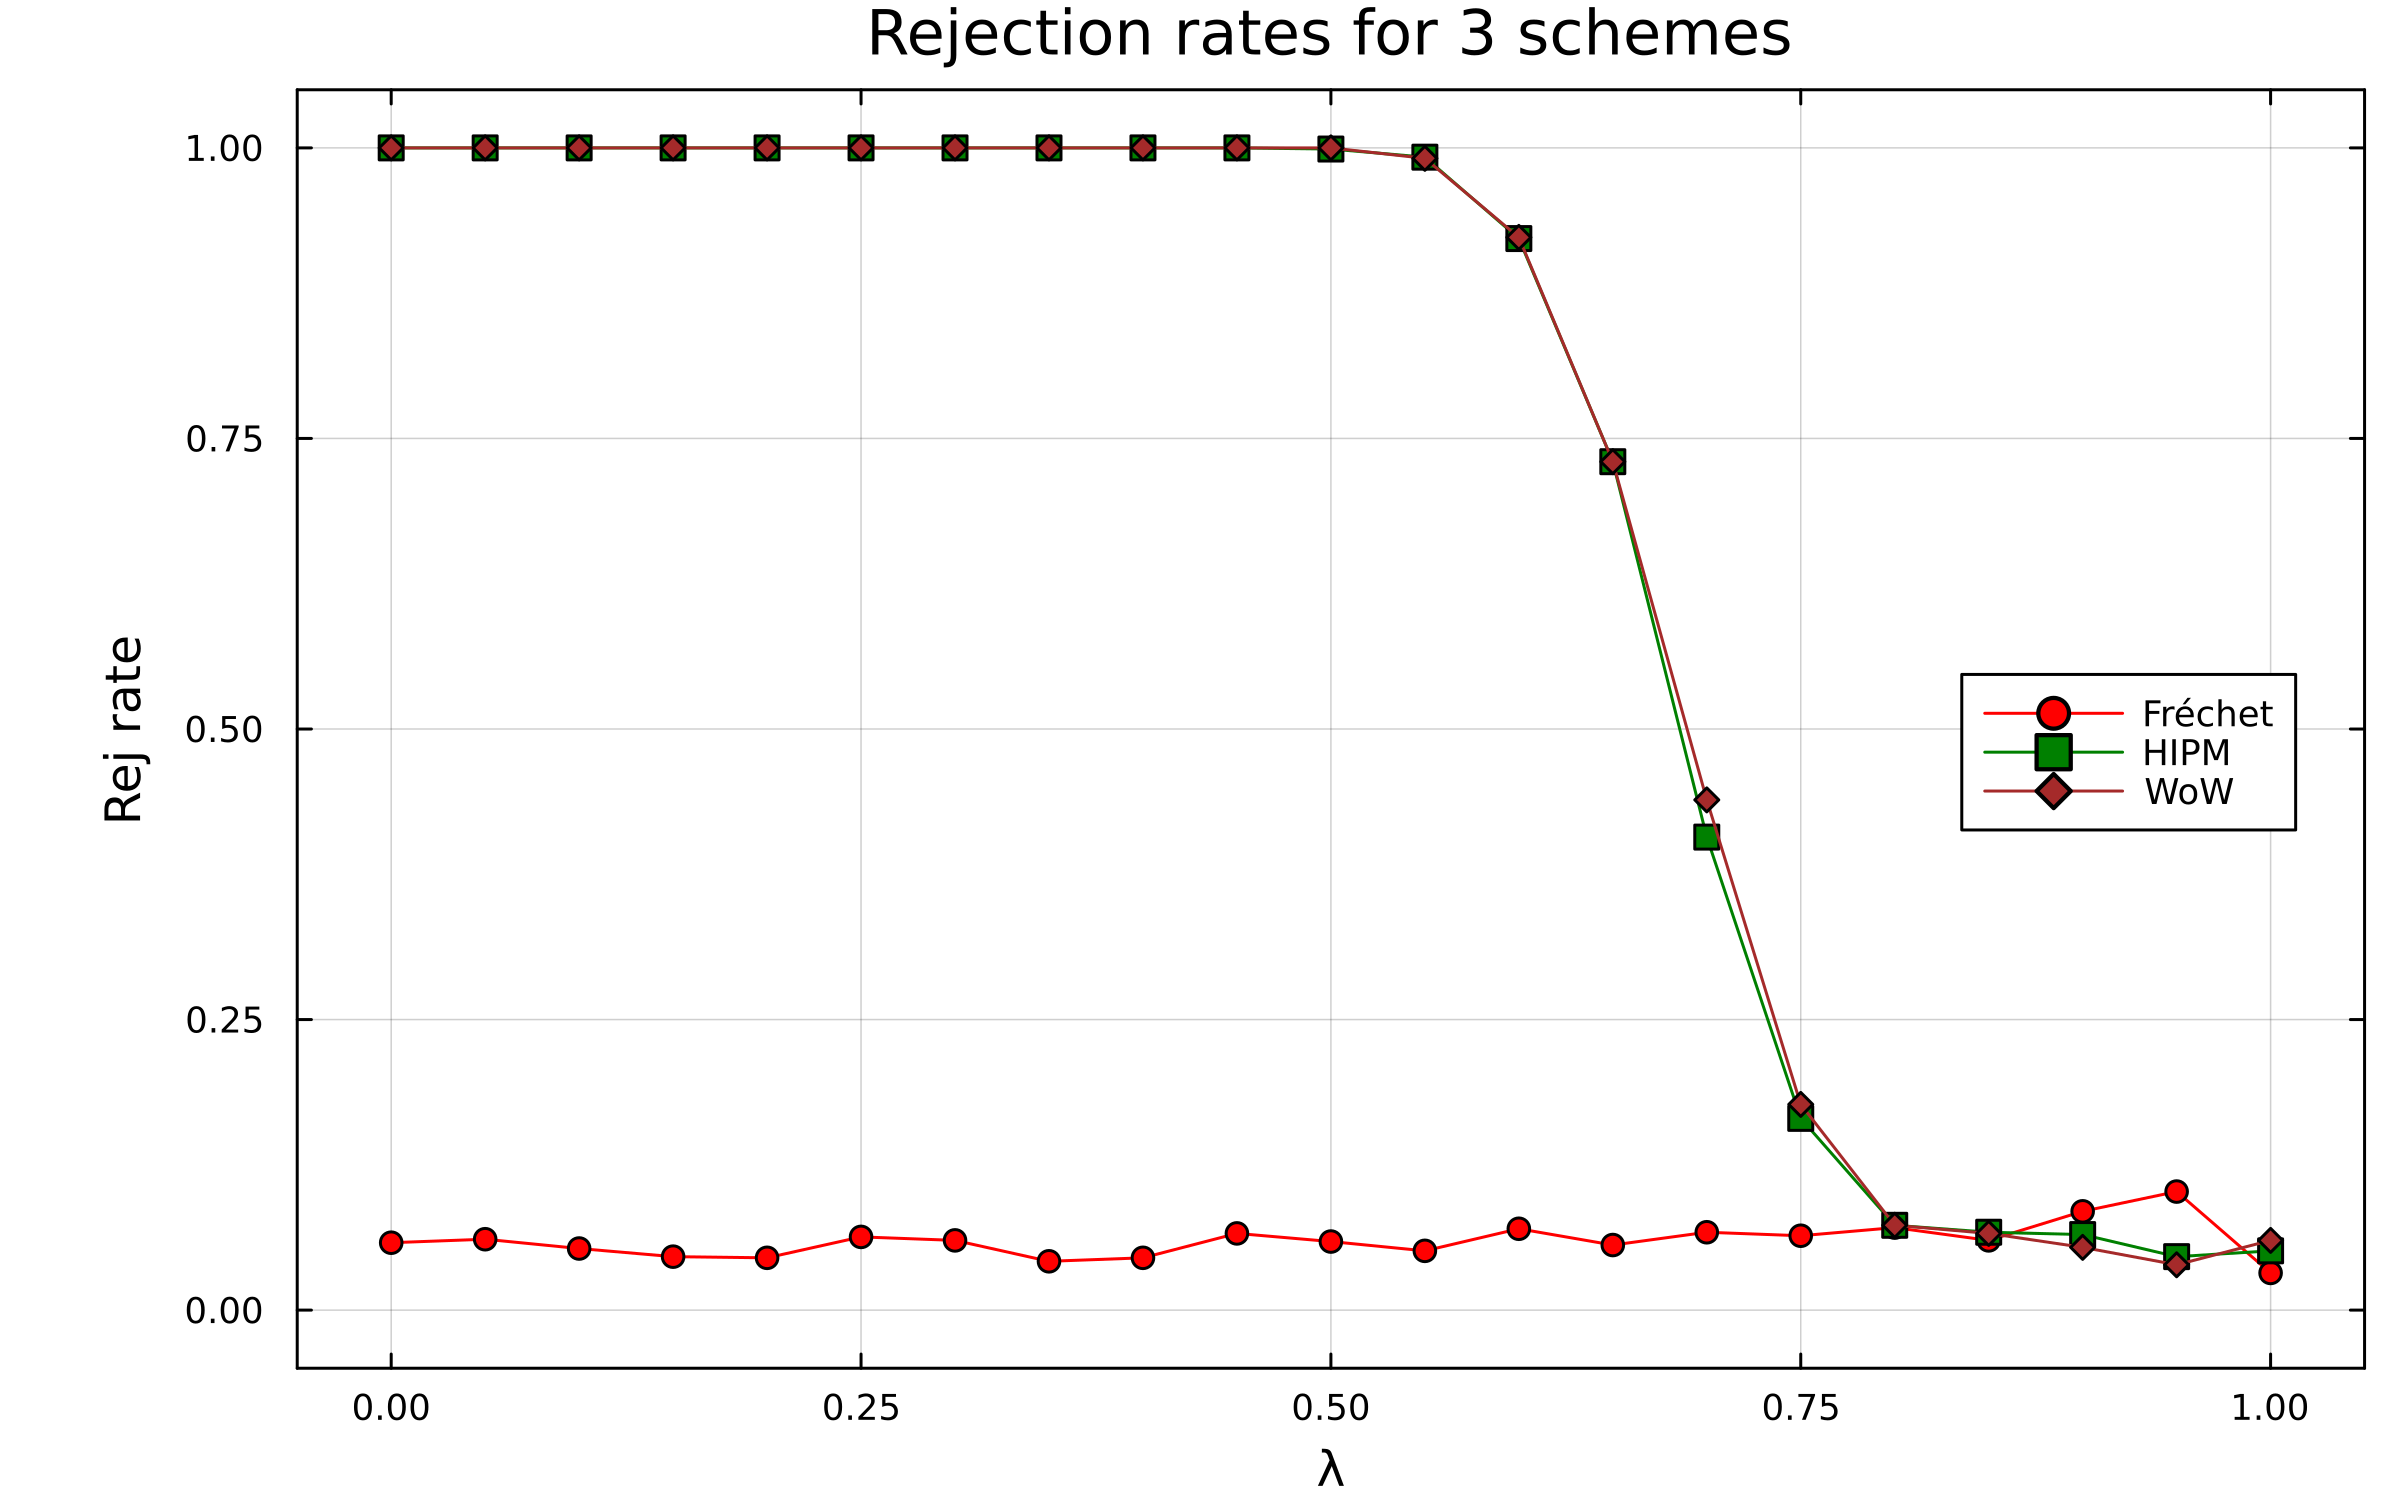
\includegraphics[width=0.43\textwidth]{chapters/two-sample-testing/figures/all_schemes/counterexample_n=100_m=200_S=1000_bootstrap=false_n_samples=100.png}
    \caption{Rejection rates for WoW, HIPM, Fr\'echet and Energy tests}
    \label{figure:counterexample}
\end{figure}

As observed in Figure~\ref{figure:counterexample}, since the two distributions induce the same Fr\'echet means and variances, the method proposed in \cite{dubey2019frechet} fails to detect the presence of different laws. In contrast, the HIPM and WoW tests perform slightly better than the Energy test in identifying the discrepancy.

To conclude, although the Fr\'echet test can exhibit higher power than the other testing schemes in certain settings, its main limitation is that it fails to detect the difference when the laws of random probability measures are not fully characterized by the Fr\'echet mean and variance. The Energy test, as well as permutation tests based on HIPM or WoW, mitigate this limitation. Moreover, HIPM and WoW may be preferable to the Energy test in practice, since the underlying metric space, in our case, the space of probability measures, may fail to be of strongly negative type, or this property may be difficult to verify.


\subsection{Mortality Data}\label{subsection:mortality_data}

We apply our proposed testing scheme to human mortality data obtained from the Human Mortality Database (https://www.mortality.org/). The dataset contains period life tables for various countries and calendar years. A period life table summarizes mortality conditions in a given calendar year by describing how a hypothetical cohort would die if it faced the age-specific mortality proportions observed in that year. The resulting mortality proportions are then used to derive the age-at-death distribution of the hypothetical cohort.

Our analysis compares mortality proportions from 1960 to 2010 between two historically motivated groups of countries. Following the classification in \cite{dubey2019frechet}, the first group consists of countries that were either part of the Soviet Union or belonged to the Soviet-aligned Eastern Bloc during much of the 20th century. The second group consists mainly of Western or non-Soviet high-income countries, including several countries that were politically neutral during the Cold War.
\begin{itemize}
    \item Group 1 : Belarus, Bulgaria, Czechia, Estonia, Hungary, Latvia, Lithuania, Poland, Russia, Slovakia, and Ukraine.
    \item Group 2 : Australia, Austria, Belgium, Canada, Denmark, Finland, France, Iceland, Ireland, Italy, Japan, Luxembourg, Netherlands, New Zealand, Norway, Spain, Sweden, Switzerland, United Kingdom, and United States of America.
\end{itemize}
The age range is $\{0,1,\cdots,110\}$, where $110$ denotes that death occurred at that age or later. We choose not to truncate the age range for the following reasons. First, visual inspection of the probability mass functions and quantiles does not reveal any abnormalities, particularly at higher ages (see Figure~\ref{figure:quantile_for_mortality_rates}). Second, truncating the age range leads to significant data loss. For example, among females, the maximum percentage of data lost across countries is at least $20$ percent for all time periods when the age interval is truncated to $\{0,1,\dots,85\}$.

In Figure~\ref{figure:quantile_for_mortality_rates}, we present the quantile plots of the probability mass functions corresponding to age at death for both males and females. We consider the years 1960, 1992, and 2008 to capture different historical periods: the Cold War era closer to the post-war period, the years shortly after the collapse of the Soviet Union, and a more recent period following the breakup. The plots are shown separately for females and males. As observed, noticeable differences can be visually identified, particularly in the more recent time periods.
\begin{figure}[htbp]
    \centering
    \begin{subfigure}{0.5\textwidth} % Increased width since they are stacked
        \centering
        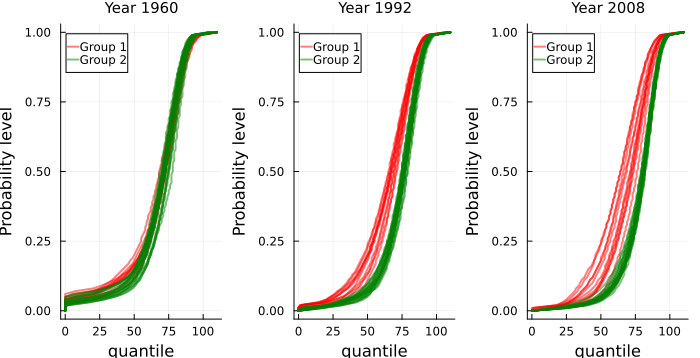
\includegraphics[width=\linewidth]{chapters/two-sample-testing/figures/mortality/males_allquantiles_0_110.png}
        \caption{Males}
    \end{subfigure}
    \\ % <--- This line break forces the next subfigure down
    \begin{subfigure}{0.5\textwidth}
        \centering
        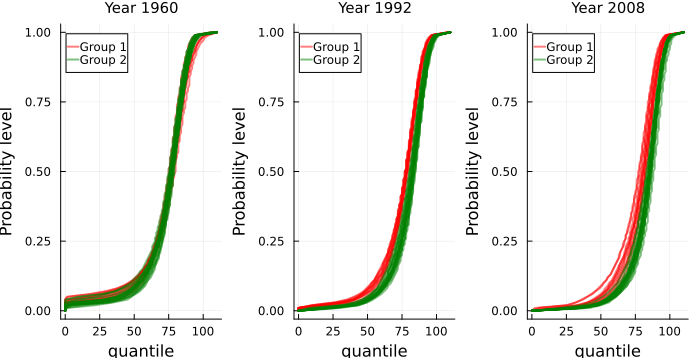
\includegraphics[width=\linewidth]{chapters/two-sample-testing/figures/mortality/females_allquantiles_0_110.png}
        \caption{Females}
    \end{subfigure}
    \caption{Quantile plots of the age-at-death probability mass functions for the two country groups}
    \label{figure:quantile_for_mortality_rates}
\end{figure}
To assess whether there is a difference in mortality proportions between the two groups of countries in each time period, we apply tests using HIPM and WoW separately for males and females. We set the significance level to $\theta = 0.05$ and use $n_{\text{perm}} = 100$ permutations to compute a p-value for each year.

We also compare the p-values obtained from our approach with those derived from the following alternative methods:
\begin{itemize}
\item Averaging: Given $\widehat{P}^1_1,\cdots, \widehat{P}^1_{n_1}$ from group 1 and $\widehat{P}^2_1,\cdots, \widehat{P}^2_{n_2}$ from group 2, we obtain average probability measures inside each group, i.e.
\[
\overline{P}^1 = \frac{1}{n_1}\sum_{i = 1}^{n_1}\widehat{P}^1_i, \quad
\overline{P}^2 = \frac{1}{n_2}\sum_{i = 1}^{n_2}\widehat{P}^2_i.
\]
The test statistic is obtained by computing Wasserstein-1 distance between $\overline{P}^1$ and $\overline{P}^2.$ The threshold is obtained via a permutation approach, in which the observed probability measures are permuted across the two groups.
\item Pooling: This approach is included to emphasize the importance of preserving the probability-measure structure within each group. Since the goal is to compare mortality proportions across the two groups, one might instead ignore the country-level distributional structure and simply aggregate deaths within each group. This aggregation produces a single probability measure for each group, and the test statistic is then computed as the Wasserstein-1 distance between these two measures. As before, the significance threshold is obtained using a permutation procedure. Because the data for each country consist of death counts by age, we first convert these counts into observations of age at death. Specifically, if there are $k$ deaths at age $a$, we generate $k$ observations equal to $a$. This is done separately for each group. The resulting age-at-death observations are then permuted across the two groups, which allows the permutation procedure to operate directly on individual age-at-death observations rather than on aggregated counts.
\end{itemize}
Note that the test statistic is identical for both the pooling and averaging approaches; the difference between the two testing schemes lies in the permutation procedure. In particular, the averaging approach preserves the probability measure structure within each group, whereas the pooling approach does not.

Examining the p-values from all methods in Figure~\ref{figure::p_values_mortality}, we observe that for females, the difference between the groups is statistically significant in 1960. During the following decade, this difference becomes less significant under the methods based on HIPM, WoW, and Averaging, which may be explained by economic growth. After the 1970s, the disparity in mortality proportions between the groups increases again, potentially reflecting the economic decline in the countries of Group~1. Following the breakup of the Soviet Union, the observed differences may be associated with countries that were unable to integrate well into the Western bloc.

A similar trend is observed for males; however, the key difference is that during the period from 1960 to 1970, although the differences in mortality proportions were decreasing, this was not statistically significant in all of those years.
\begin{figure}[htbp]
    \centering
    \begin{subfigure}{0.5\textwidth} % Increased width since they are stacked
        \centering
        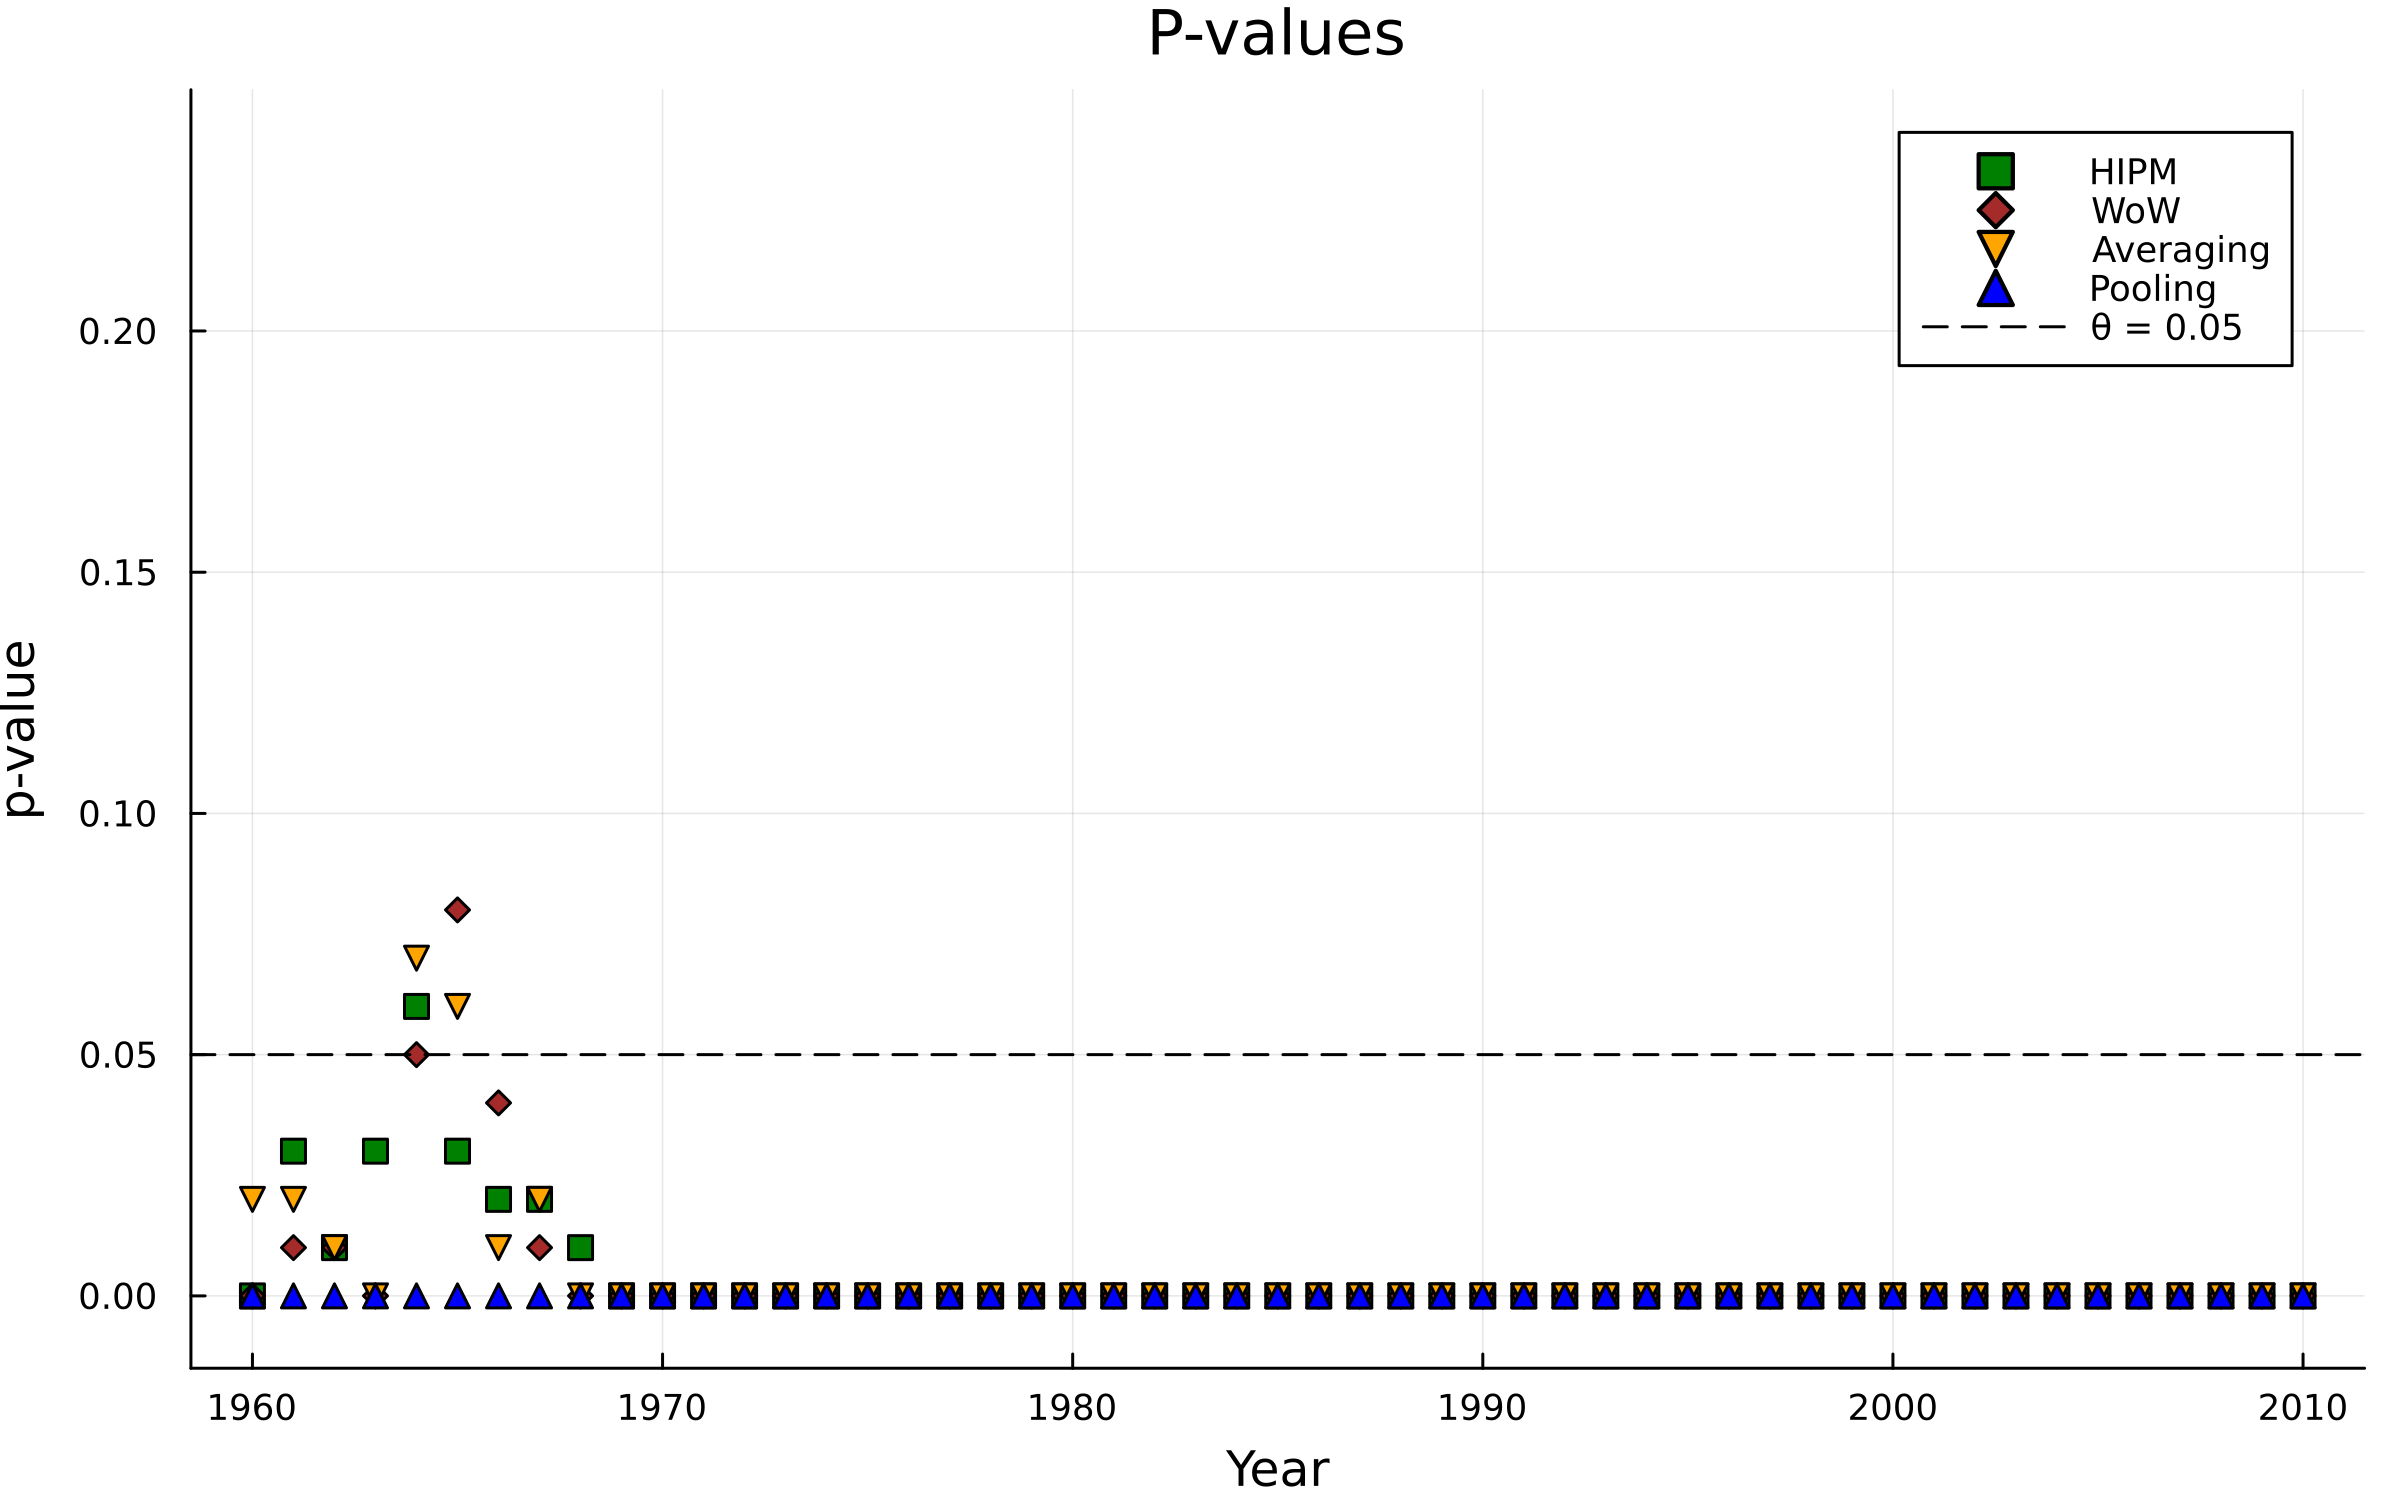
\includegraphics[width=\linewidth]{chapters/two-sample-testing/figures/mortality/pvalues_males.png}
        \caption{Males}
    \end{subfigure}
    \\ % <--- This line break forces the next subfigure down
    \begin{subfigure}{0.5\textwidth}
        \centering
        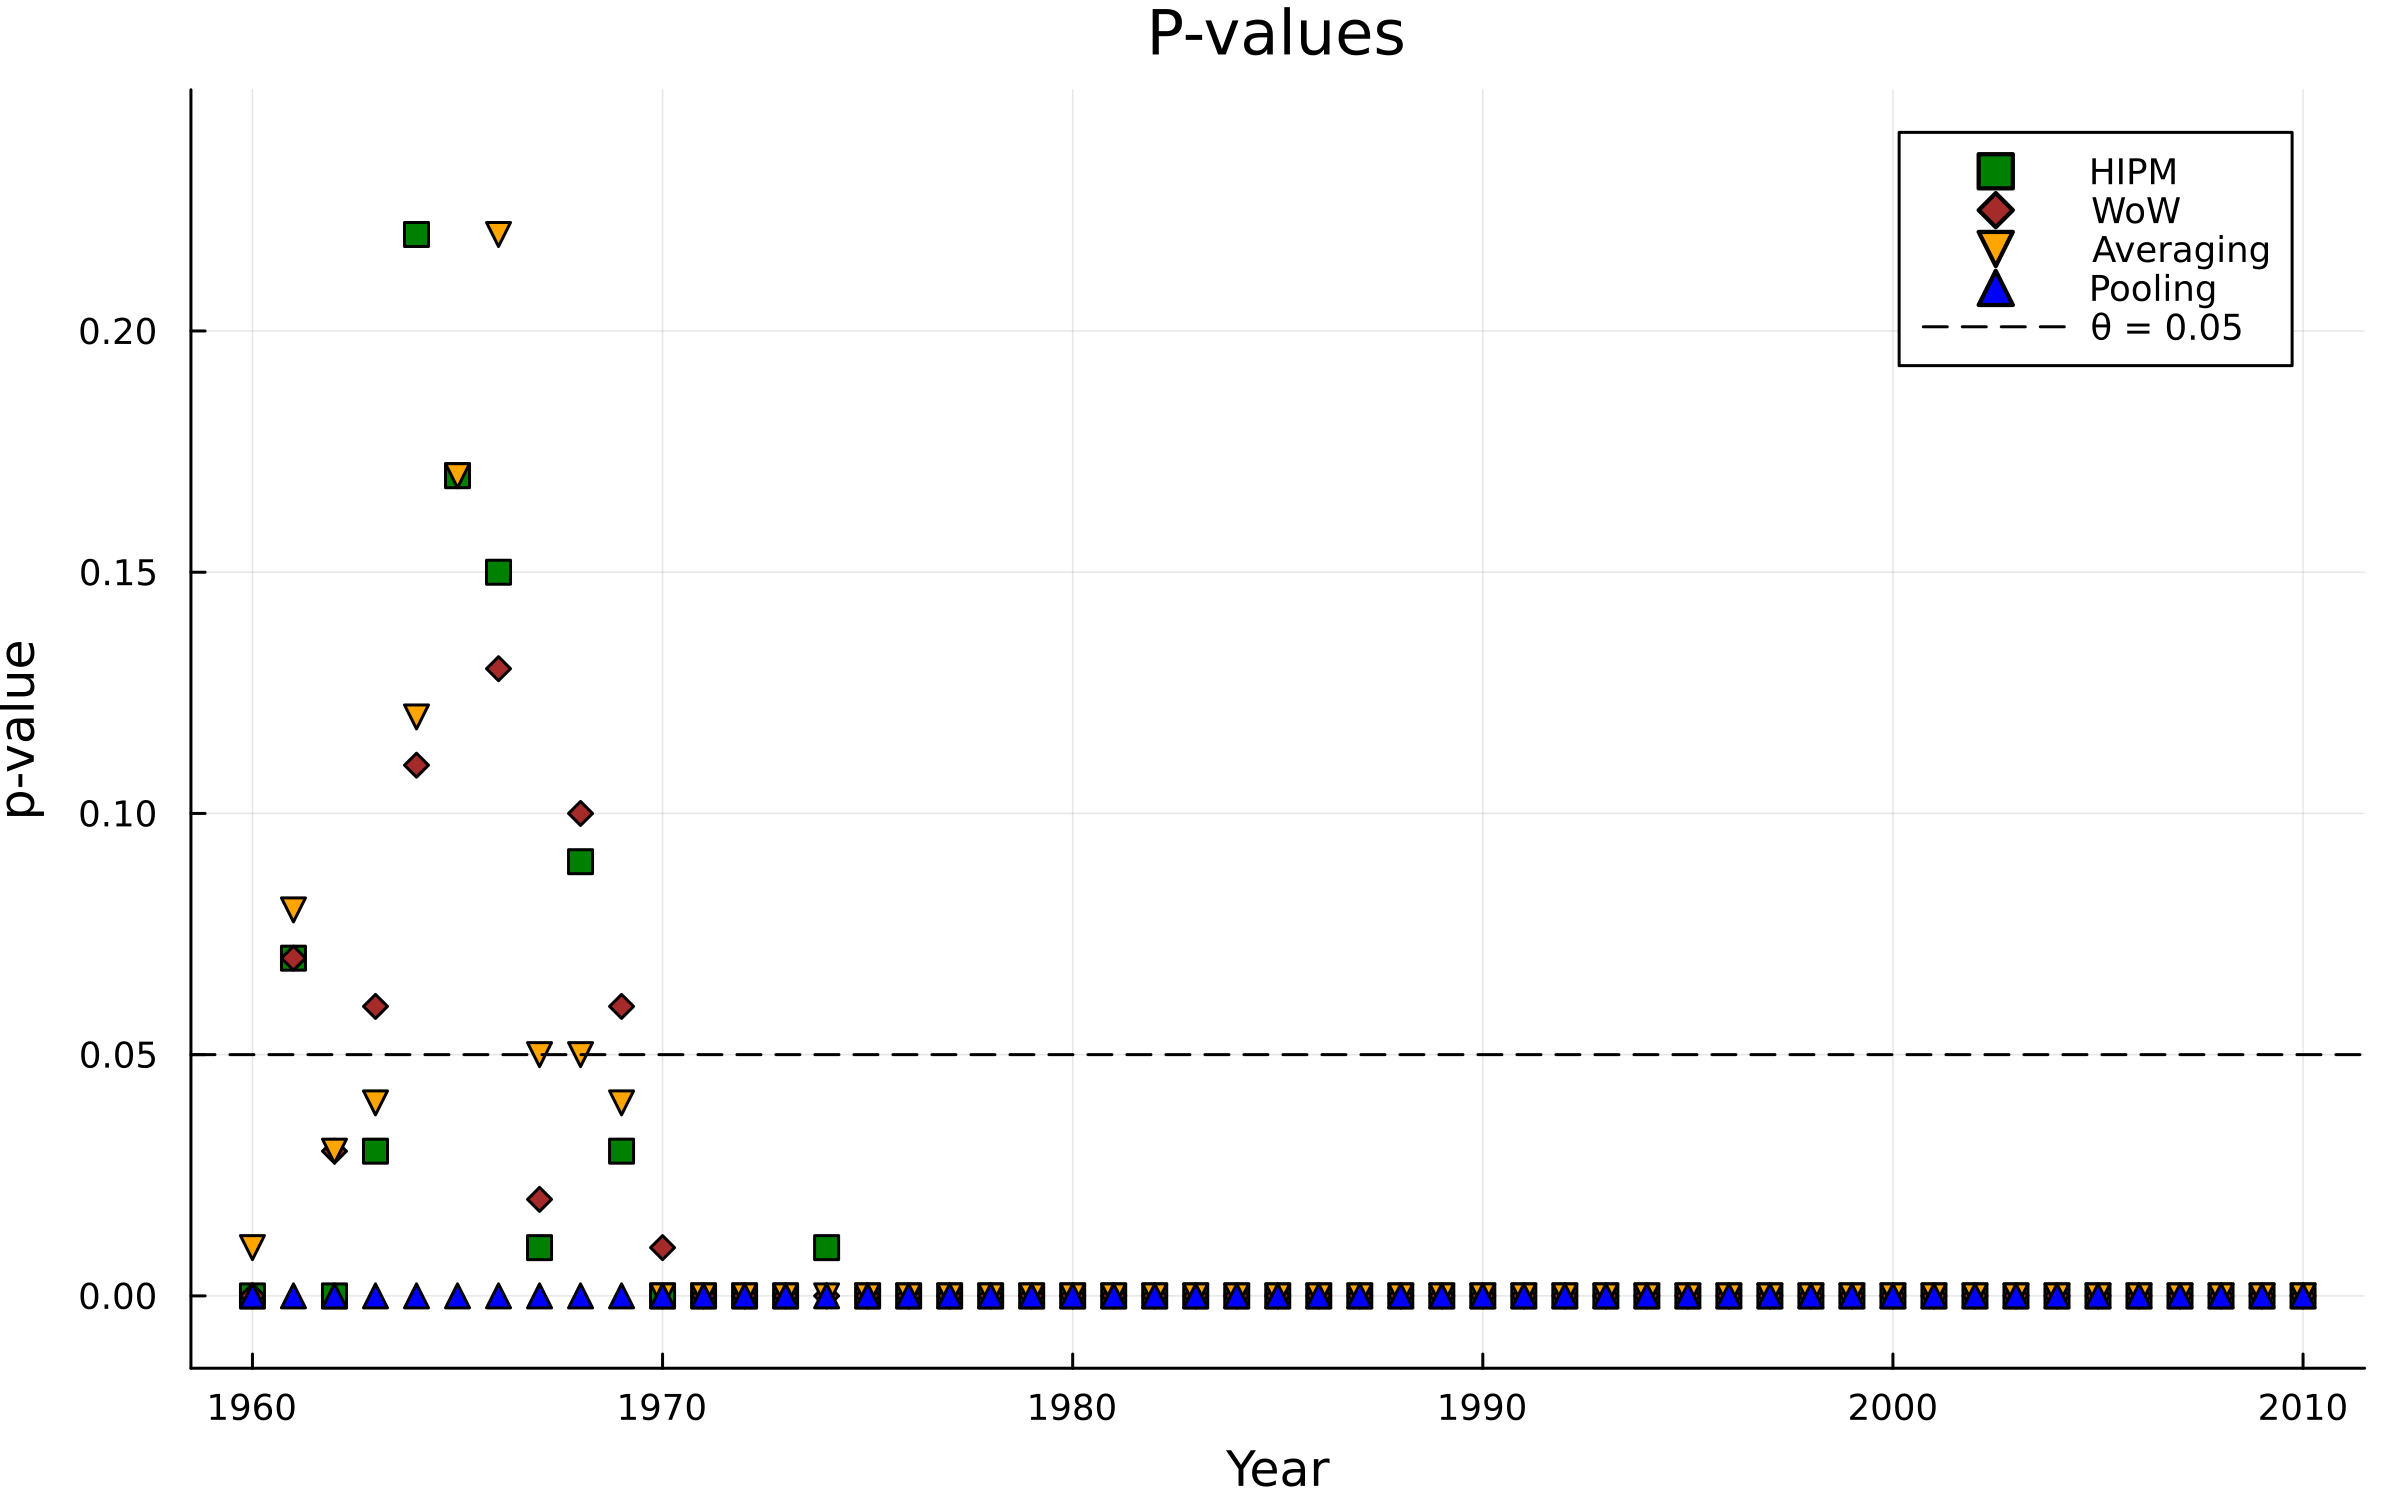
\includegraphics[width=\linewidth]{chapters/two-sample-testing/figures/mortality/pvalues_females.png}
        \caption{Females}
    \end{subfigure}
    \caption{P-values for mortality proportions}
    \label{figure::p_values_mortality}
\end{figure}

Note also that the p-values for Averaging, HIPM, and WoW follow a similar trend. This is because the average measure is in this case sufficient to detect the difference between the two groups.


We also observe an important issue concerning the pooling approach, which is of broader relevance to hierarchical sampling settings. In particular, the pooling procedure may fail to control the Type I error in hierarchical sampling settings. This is because pooling ignores the fact that observations within each country are generated from a latent random probability measure. Under hierarchical sampling, where we observe $n$ sequences of length $m$, each generated from a different latent random probability measure, the empirical distribution obtained by pooling all observations converges to the mean measure of the law of the random probability measure. Hence, the pooled test statistic converges to the Wasserstein distance between the two group-level mean measures. In contrast, the permutation samples behave as if they were drawn directly from this mean measure, with an effective sample size of $nm$. As a result, the permutation threshold converges to zero faster than the observed distance, leading to systematically small p-values. This issue disappears when the latent probability measures are identical.











        
        


        
      


        
       


        







